%%This is a very basic article template.
%%There is just one section and two subsections.
\documentclass{article}
\usepackage{graphicx}
\usepackage{amsmath}
\usepackage{mathtools}
\newcommand{\east}{e_e}
\newcommand{\north}{e_n}
\newcommand{\up}{e_n}
\newcommand{\range}{e_r}
\newcommand{\bearing}{e_\theta}
\newcommand{\elevation}{e_\phi}
\newcommand{\rrate}{\dot{r}}
\newcommand{\brate}{\dot{\theta}}
\newcommand{\erate}{\dot{\phi}}
\newcommand{\carvec}{\hat{e_{c}}}
\newcommand{\polvec}{\hat{e_{p}}}


\begin{document}

\section{Coordinate Conversions}

\subsection{Spherical Coordinate system}
In the polar coordinate system we represent the location of the target in terms
of range, bearing and elevation. where range denotes the distance away from the
target's position, bearing denotes the angle to the target (taken from the north
axis), and elevation denotes the angle between the tanget plan and the target.

\begin{figure}[h]\label{fig:spherical}
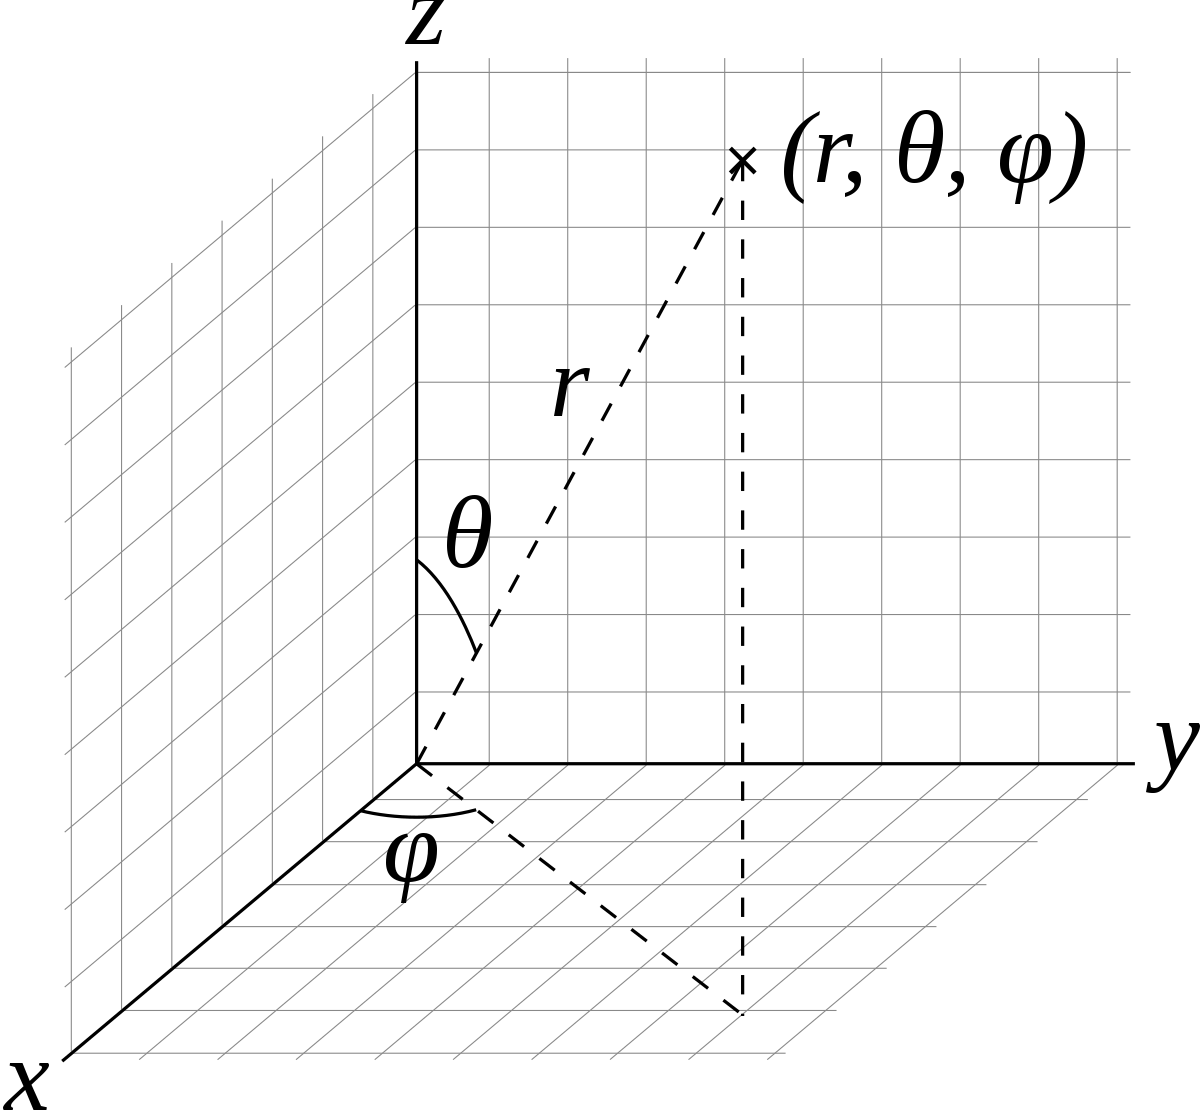
\includegraphics[width=0.5\textwidth,height=0.5\textheight,keepaspectratio]{figures/spherical}
\end{figure}

\subsection{Cooridnate system representation}

We denote by $\carvec=(\east,\north, \up)$ the column vector that represents
the the coordinate system in ENU terms. each $\east,\north, \up$ is a unit vector
which represents the distance in east direction, north direction and up
direction, respectively.

We denote by $\polvec=(\range,\bearing,\elevation)$ the column vector that
represents the the coordinate system in spherical terms. each $\range,\bearing,\elevation$ is a
unit vector which represents the distance in east direction, north direction and up
direction, respectively.

\subsection{Conversion from one system to the other}

Let $\vec{p} = (x,y,z) \cdot \carvec = x\east + y\north + z\up$ denote the
position of the target. We would like to convert the vector $\carvec$ to spherical
coordinates $\polvec$.
Clearly, for the position we have:

\begin{align}
\begin{split}
{}& x=r\sin \theta \cos \phi \\
{}& y=r\cos \theta \cos \phi \\
{}& z=r\sin \phi
\end{split}
\end{align}

That is, $\vec{p} = r\sin \theta \cos \phi \east + r\cos \theta \cos \phi \north +
r\sin \phi \up = r( \sin \theta \cos \phi \east + \cos \theta \cos \phi \north +
\sin \phi \up)$

\begin{equation}
\vec{p} = r( \sin \theta \cos \phi \east + \cos \theta \cos \phi \north +
\sin \phi \up)
\end{equation}

And we obtain:
\begin{equation}\label{eq:range}
\range = \frac{\frac{\partial \vec{p}}{\partial r}}{\| \frac{\partial
\vec{p}}{\partial r} \|} = \sin \theta \cos \phi \east + \cos \theta \cos \phi \north +
\sin \phi \up 
\end{equation}

\begin{align}\label{eq:bearing}
\begin{split}
\bearing = \frac{\frac{\partial \vec{p}}{\partial \theta}}{\| \frac{\partial
\vec{p}}{\partial \theta} \|} = \frac{r( \cos \theta \cos \phi \east - \sin
\theta \cos \phi \north) }{r \| \cos \theta \cos \phi \east - \sin \theta
\cos \phi \north\|} = \\
= \frac{r( \cos \theta \cos \phi \east - \sin \theta
\cos \phi \north) }{r |\cos \phi |} = \cos \theta \east - \sin \theta \north
\end{split}
\end{align}

\begin{align}
\begin{split}
\elevation = \frac{\frac{\partial \vec{p}}{\partial \phi}}{\| \frac{\partial
\vec{p}}{\partial \phi} \|} = \frac{r( - \sin \theta \sin \phi \east - \cos
\theta \sin \phi \north + \cos \phi \up) }{r \| - \sin \theta \sin \phi \east - \cos
\theta \sin \phi \north + \cos \phi \up \|} = \\
= \frac{r( - \sin \theta \sin \phi \east - \cos
\theta \sin \phi \north + \cos \phi \up) }{r} = \\
= - \sin \theta \sin \phi \east
- \cos \theta \sin \phi \north + \cos \phi \up
\end{split}
\end{align}

Namely,

\begin{equation}\label{eq:matrix}
\begin{pmatrix}
    \range \\
   \bearing \\
    \elevation
  \end{pmatrix}
  \qquad
  = \begin{pmatrix}
    \sin \theta \cos \phi & \cos \theta \cos \phi &  \sin \phi \\
   \cos \theta &  -\sin \theta & 0 \\
    -\sin \theta \sin \phi & -\cos \theta \sin \phi &  \cos \phi
  \end{pmatrix}
  \qquad
  \begin{pmatrix}
    \east \\
   \north \\
    \up
  \end{pmatrix}
\end{equation}

In Equation~\ref{eq:bearing} we canceled the term $\cos \phi$
since it is always positive $\| \cos \phi \| = \cos \phi$.

Denote by $\Sigma$ the conversion matrix as described above, note that $\Sigma$
is unitary matrix.

\begin{equation}
\Sigma^{-1} = \begin{pmatrix}
    \sin \theta \cos \phi & \cos \theta &  - \sin \theta \sin \phi \\
   \cos \theta \cos \phi &  -\sin \theta & -\cos \theta \sin \phi \\
    \sin \phi & 0 &  \cos \phi
  \end{pmatrix}
\end{equation}

\subsection{Velocity conversion}
Let $\vec{v}$ denote the velocity vector. We denote by $\rrate, \brate, \erate$ the terms: range-rate, bearing-rate,
elevation-rate.
In spherical coordinate system, the
following equation holds:
\begin{equation}
\vec{v} = \frac{d}{dt} (r(t) \range)
\end{equation}

By the chain-rule: $\frac{d}{dt} (r(t) \range) = \rrate \range + r(t)
\frac{d}{dt} \range$.

For the left term we have:

\begin{align*}
\begin{split}
& \frac{d}{dt} \range = \frac{d}{dt}(\sin \theta \cos \phi \east + \cos \theta
\cos \phi \north + \sin \phi \up ) =  \\ 
& \brate \cos \theta \cos \phi \east -
\erate \sin \theta \sin \phi \east - \brate \sin \theta \cos \phi \north - \erate \cos
\theta \sin \phi \north + \erate \cos \phi \up = \\
& = \brate \cos \phi \bearing + \erate \elevation 
\end{split}
\end{align*}


Which concludes to:

\begin{equation}\label{eq:velocity-polar}
\vec{v} = \rrate \range + r \brate \cos \phi \bearing + r \erate \elevation 
\end{equation}

\subsection{Conversion from spherical to cartesian}
Using Equations~\ref{eq:matrix} and~\ref{eq:velocity-polar}, we deduce:


\begin{equation}\label{eq:car-polar}
\begin{pmatrix}
    v_x \\
   v_y \\
    v_z
  \end{pmatrix}
  \qquad
  = \begin{pmatrix}
    \rrate & \brate \cos \phi & \erate
  \end{pmatrix}
  \qquad
  \begin{pmatrix}
    \range \\
   \bearing \\
    \elevation
  \end{pmatrix}
  = \begin{pmatrix}
    \rrate & \brate \cos \phi & \erate
  \end{pmatrix} (\Sigma \carvec)
\end{equation}


\end{document}
